\documentclass[12pt]{article} %font size 12pt
\usepackage[a4paper, margin=1in]{geometry} %a4 size margin=1 inch
\usepackage{graphicx} % Required for inserting images
\usepackage{changepage}
\linespread{1} %single line spacing
\bibliographystyle{plain}
\usepackage{rotating}
\usepackage{tikz}
\DeclareUnicodeCharacter{2060}{\nolinebreak}
\usetikzlibrary{mindmap, shapes, arrows.meta, positioning}
\usepackage{pgfgantt}
\usepackage{appendix}
\usepackage{svg}
\usepackage{tabularx}
\usepackage{dblfloatfix}
\usepackage[utf8]{inputenc}
\usepackage{graphicx}
\graphicspath{ {figures/} }
\usepackage{array}
\usepackage{color}   %May be necessary if you want to color links
\usepackage{setspace}
\usepackage{hyperref}
\usepackage[load-configurations = abbreviations]{siunitx}
\usepackage[acronym]{glossaries}
\usepackage{imakeidx}
\makeindex[columns=3, title=Index,intoc]
\hypersetup{
    colorlinks=true, %set true if you want colored links
    linktoc=all,     %set to all if you want both sections and subsections linked
    linkcolor=blue,  % Choose some color if you want links to stand out
}

\makeglossaries
\newglossaryentry{Abrasion Resistance}
{
        name=abrasion resistance,
        description={Abrasion Resistance refers to the ability of a material to withstand wear, rubbing, or friction, maintaining its surface integrity and resisting damage caused by repeated contact with abrasive forces or surfaces}
}
\newglossaryentry{Tear Strength}
{
        name=tear strength,
        description={Tear Strength is a measure of a material's resistance to tearing or the force required to propagate a tear, indicating its durability against the initiation and growth of a tear or cut}
}
\newglossaryentry{Seam Slippage}
{
        name=seam slippage,
        description={Seam spillage is the undesired leakage of contents through container seams due to inadequate sealing, posing a risk of material loss}
}
\newglossaryentry{Denier}
{
        name=denier,
        description={Denier is a unit of measurement for the linear mass density of fibers, indicating the weight in grams of a 9,000-meter length, commonly used to express the thickness or fineness of yarn in the textile industry}
}
\newglossaryentry{Cleaning Efficacy}
{
        name=cleaning efficacy,
        description={The effectiveness of a cleaning process in removing dirt, stains, and other contaminants from fabrics}
}
\newglossaryentry{thread count}
{
        name=thread count,
        description={The number of threads woven into a square inch of fabric}
}
\newglossaryentry{Colorfastness}
{
        name=denier,
        description={The ability of a fabric to resist fading or bleeding color when exposed to light, water, or other laundering agents}
}
\newglossaryentry{Tensile Method Test}
{
        name=tensile method test,
        description={A test that measures the breaking strength of a fabric by pulling it until it breaks}
}
\newglossaryentry{back-folded seams}
{
        name=back-folded seams,
        description={A type of seam where the raw edges of the fabric are folded back and sewn together}
}
\newglossaryentry{wet cleaning agent}
{
        name=wet cleaning agent,
        description={A detergent or solvent specifically designed and used for wet cleaning}
}
\newglossaryentry{tumble drying process}
{
        name=tumble drying process,
        description={A drying method that uses a rotating drum to circulate hot air around fabrics}
}
\newglossaryentry{access panel}
{
        name=Access panels,
        description={A removable panel on a machine that allows for access to its internal components for cleaning or maintenance}
}
\newglossaryentry{effluent treatment}
{
        name=effluent treatment,
        description={The process of removing pollutants from wastewater before it is released back into the environment}
}
\newglossaryentry{pre-spotting agents}
{
        name=pre-spotting agents,
        description={Cleaning agents that are applied directly to stains before washing to help break them down and make them easier to remove}
}

\newacronym{if}{IF}{Involvement Factor}
\newacronym{ac}{AC}{Activity Coordinator}
\newacronym{tc}{TC}{Tribe Coordinator}
\newacronym{WBS}{WBS}{Work Breakdown Structure}
\newacronym{plc}{PLC}{Programmable Logic Controller}
\newacronym{hmi}{HMI}{Human-Machine Interface}
\newacronym{cpcb}{CPCB}{Central Pollution Control Board}
\newacronym{perc}{PERC}{Perchloroethylene}
\newacronym{cad}{CAD}{Computer-Aided Design}
\newacronym{cfm}{CFM}{Cubic Feet Per Minute}
\newacronym{hdpe}{HDPE}{High Density Polyethylene}
\newacronym{pvc}{PVC}{Polyvinyl Chloride}
\newacronym{TRL}{TRL}{Technology Readiness Level}
\newacronym{seac}{SEAC}{Surf Excel’s Safety and Environmental Assurance Centre}


\begin{document}
\begin{titlepage}
\thispagestyle{empty}
\centering

\includegraphics[width=0.3\textwidth]{logo.png}
\vfill
\centering
\vspace{10pt}
\setstretch{2}
{\huge\textbf{ELP305-Submission-02:\\ Cleaning Machine Requirements and Specifications}}



\vspace{1cm}
\Huge\textbf{}
\vspace{1cm}
\vfill
\huge\textit{Tribe B}
\end{titlepage}



\clearpage
\section*{Tribe B Team Member Details}
\subsection{Tribe B Members with  \acrshort{if} = 1}
\begin{table}[h!]
\centering

\begin{tabular}{|c|c|c|c|c|}
\hline
Name & Entry No & Email & Role & \acrshort{if} \\
\hline
Aditya Arya & 2021MT60958 & \href{mailto:mt6210958@maths.iitd.ac.in}{mt6210958@maths.iitd.ac.in} & \acrshort{tc} & 1 \\
Ark Verma & 2021EE10783 & \href{mailto:ee1210783@ee.iitd.ac.in}{ee1210783@ee.iitd.ac.in} & \acrshort{tc} & 1 \\
\hline
\end{tabular}
\caption{Tribe Coordinator Details}
\label{tab:teamDetails}
\end{table}

\begin{table}[h!]
\centering
\begin{tabular}{|c|c|c|c|c|}
\hline
Name & Entry No & Email & Role & \acrshort{if} \\
\hline
Bhumi Gadhavi & 2021MT60950 & \href{mailto:mt6210950@maths.iitd.ac.in}{mt6210950@maths.iitd.ac.in} & \acrshort{ac} & 1 \\
Tanmay Jhalani & 2021EE30389 & \href{mailto:ee3210389@ee.iitd.ac.in}{ee3210389@ee.iitd.ac.in} & Member & 1 \\
Shantanu Pandit & 2021MT10252 & \href{mailto:mt1210252@maths.iitd.ac.in}{mt1210252@maths.iitd.ac.in} & Member & 1 \\
Advait Prashant Rege & 2021MT60946 & \href{mailto:mt6210946@maths.iitd.ac.in}{mt6210946@maths.iitd.ac.in} & Member & 1 \\
Pramsu Shrivastava & 2021EE10140 & \href{mailto:ee1210140@ee.iitd.ac.in}{ee1210140@ee.iitd.ac.in} & Member & 1 \\
Parth Naikwad & 2021EE10672 & \href{mailto:ee1210672@ee.iitd.ac.in}{ee1210672@ee.iitd.ac.in} & Member & 1 \\
Yash Bafna & 2021EE10660 & \href{mailto:ee1210660@ee.iitd.ac.in}{ee1210660@ee.iitd.ac.in} & Member & 1 \\
Abhay Yadav & 2021EE10151 & \href{mailto:ee1210151@ee.iitd.ac.in}{ee1210151@ee.iitd.ac.in} & Member & 1 \\
Ram Gopal Chaudhari & 2021EE10671 & \href{mailto:ee1210671@ee.iitd.ac.in}{ee1210671@ee.iitd.ac.in} & Member & 1 \\
Vivek Pratap Singh & 2021EE10687 & \href{mailto:ee1210687@ee.iitd.ac.in}{ee1210687@ee.iitd.ac.in} & Member & 1 \\
Shreya Gupta & 2021MT10906 & \href{mailto:mt1210906@maths.iitd.ac.in}{mt1210906@maths.iitd.ac.in} & Member & 1 \\
Vaibhav & 2021EE10641 & \href{mailto:ee1210641@ee.iitd.ac.in}{ee1210641@ee.iitd.ac.in} & Member & 1 \\
Devanshu Ataria & 2021EE10162 & \href{mailto:ee1210162@ee.iitd.ac.in}{ee1210162@ee.iitd.ac.in} & Member & 1 \\
Anmol Bansal & 2021EE10643 & \href{mailto:ee1210643@ee.iitd.ac.in}{ee1210643@ee.iitd.ac.in} & Member & 1 \\
Vedant Patel & 2020EE10520 & \href{mailto:ee1200520@ee.iitd.ac.in}{ee1200520@ee.iitd.ac.in} & Member & 1 \\
Aditi Srivastava & 2021MT10228 & \href{mailto:mt1210228@maths.iitd.ac.in}{mt1210228@maths.iitd.ac.in} & Member & 1 \\
Anusha Kedawat & 2021EE30718 & \href{mailto:ee3210718@ee.iitd.ac.in}{ee3210718@ee.iitd.ac.in} & Member & 1 \\
Manan Singal & 2021EE10138 & \href{mailto:ee1210138@ee.iitd.ac.in}{ee1210138@ee.iitd.ac.in} & Member & 1 \\
Tanisha Chouhan & 2021EE10693 & \href{mailto:ee1210693@ee.iitd.ac.in}{ee1210693@ee.iitd.ac.in} & Member & 1 \\
Vedant Kokate & 2021EE10631 & \href{mailto:ee1210631@ee.iitd.ac.in}{ee1210631@ee.iitd.ac.in} & Member & 1 \\
Subham & 2022MT11823 & \href{mailto:mt1221823@maths.iitd.ac.in}{mt1221823@maths.iitd.ac.in} & Member & 1 \\
Siddharth  & 2022MT62028 & \href{mailto:mt6222028@maths.iitd.ac.in}{mt6222028@maths.iitd.ac.in} & Member & 1 \\
\hline
\end{tabular}
\caption{Design Team Members Details with \acrshort{if} = 1}
\label{tab:teamDetails}
\end{table}

\begin{table}[h!]
\centering
\begin{tabular}{|c|c|c|c|c|}
\hline
Name & Entry No & Email & Role & \acrshort{if} \\
\hline
Shourya Vir Jain & 2022EE31798 & \href{mailto:ee3221798@ee.iitd.ac.in}{ee3221798@ee.iitd.ac.in} & \acrshort{ac} & 1 \\
S Anuj Karthik & 2021EE10667 & \href{mailto:ee1210667@ee.iitd.ac.in}{ee1210667@ee.iitd.ac.in} & Member & 1 \\
Shreya Singla & 2020EE10671 & \href{mailto:ee1200671@ee.iitd.ac.in}{ee1200671@ee.iitd.ac.in} & Member & 1 \\
Gourab Raj Sabat & 2022EE11675 & \href{mailto:ee1221675@ee.iitd.ac.in}{ee1221675@ee.iitd.ac.in} & Member & 1 \\
Ashi Veerman & 2021MT10241 & \href{mailto:mt1210241@maths.iitd.ac.in}{mt1210241@maths.iitd.ac.in} & Member & 1 \\
Bhargab Sonowal & 2021MT10937 & \href{mailto:mt1210937@maths.iitd.ac.in}{mt1210937@maths.iitd.ac.in} & Member & 1 \\
Rakshitha & 2021MT10904 & \href{mailto:mt1210904@maths.iitd.ac.in}{mt1210904@maths.iitd.ac.in} & Member & 1 \\
Sanju N S & 2021EE30732 & \href{mailto:ee3210732@ee.iitd.ac.in}{ee3210732@ee.iitd.ac.in} & Member & 1 \\
Dhruv Joshi & 2022EE32079 & \href{mailto:ee3222079@ee.iitd.ac.in}{ee3220079@ee.iitd.ac.in} & Member & 1 \\
Drishti Gupta & 2021EE10649 & \href{mailto:ee1210649@ee.iitd.ac.in}{ee1210649@ee.iitd.ac.in} & Member & 1 \\
Deepak Kumar & 2021EE10152 & \href{mailto:ee1210152@ee.iitd.ac.in}{ee1210152@ee.iitd.ac.in} & Member & 1 \\
Varshith Reddy Ryala & 2021EE10142 & \href{mailto:ee1210142@ee.iitd.ac.in}{ee1210142@ee.iitd.ac.in} & Member & 1 \\
Raswanth J & 2021EE30179 & \href{mailto:ee3210179@ee.iitd.ac.in}{ee3210179@ee.iitd.ac.in} & Member & 1 \\
Prisha Jain & 2021EE30330 & \href{mailto:ee3210330@ee.iitd.ac.in}{ee3210330@ee.iitd.ac.in} & Member & 1 \\
Garv Gupta & 2021MT60953 & \href{mailto:mt6210953@maths.iitd.ac.in}{mt6210953@maths.iitd.ac.in} & Member & 1 \\
Dhruv Nagpal & 2020EE11013 & \href{mailto:ee1201013@ee.iitd.ac.in}{ee1201013@ee.iitd.ac.in} & Member & 1 \\
\hline
\end{tabular}
\caption{Documentation Team Members Details with \acrshort{if} = 1}
\label{tab:teamDetails}
\end{table}

\begin{table}[h!]
\centering
\begin{tabular}{|c|c|c|c|c|}
\hline
Name & Entry No & Email & Role & \acrshort{if} \\
\hline
Keshav Singhal & 2021EE10788 & \href{mailto:ee1210788@ee.iitd.ac.in}{ee1210788@ee.iitd.ac.in} & \acrshort{ac} & 1 \\
Advait Prashant Rege & 2021MT60946 & \href{mailto:mt6210946@maths.iitd.ac.in}{mt6210946@maths.iitd.ac.in} & \acrshort{ac} & 1 \\
Ridhima Gupta & 2021EE30719 & \href{mailto:ee3210719@ee.iitd.ac.in}{ee3210719@ee.iitd.ac.in} & Member & 1 \\
Diksha & 2021EE30717 & \href{mailto:ee3210717@ee.iitd.ac.in}{ee3210717@ee.iitd.ac.in} & Member & 1 \\
Tushar Daima & 2021EE10688 & \href{mailto:ee1210688@ee.iitd.ac.in}{ee1210688@ee.iitd.ac.in} & Member & 1 \\
Ridam Kumari & 2021EE10158 & \href{mailto:ee1210158@ee.iitd.ac.in}{ee1210158@ee.iitd.ac.in} & Member & 1 \\
Harsh Bagde & 2021EE10690 & \href{mailto:ee1210690@ee.iitd.ac.in}{ee1210690@ee.iitd.ac.in} & Member & 1 \\
Pratibha Patel & 2021EE10681 & \href{mailto:ee1210681@ee.iitd.ac.in}{ee1210681@ee.iitd.ac.in} & Member & 1 \\
Divyansh Bhatnagar & 2021EE30721 & \href{mailto:ee3210721@ee.iitd.ac.in}{ee3210721@ee.iitd.ac.in} & Member & 1 \\
Siddhika Tailor & 2021EE10683 & \href{mailto:ee1210683@ee.iitd.ac.in}{ee1210683@ee.iitd.ac.in} & Member & 1 \\
Dhruv Mittal & 2021EE10626 & \href{mailto:ee1210626@ee.iitd.ac.in}{ee1210626@ee.iitd.ac.in} & Member & 1 \\
\hline
\end{tabular}
\caption{Research Team Members Details with \acrshort{if} = 1}
\label{tab:teamDetails}
\end{table}

\clearpage

\subsection{Tribe B Members with  \acrshort{if} $<$ 1}

\begin{table}[h!]
\centering
\resizebox{\columnwidth}{!}{%
\begin{tabular}{|c|c|c|c|c|c|}
\hline
Name & Entry No & Email & Role & \acrshort{if} & Justification \\
\hline
Himanshu Ghusinga & 2021MT10936 & \href{mailto:mt1210936@maths.iitd.ac.in}{mt1210936@maths.iitd.ac.in} & Member & 0.5 & Hour-based formula \\
Ranjeet Mishra  & 2021EE10656 & \href{mailto:ee1210656@ee.iitd.ac.in}{ee1210656@ee.iitd.ac.in} & Member & 0.5 & Hour-based formula\\
\hline
\end{tabular}%
}
\caption{Design Team Members Details with \acrshort{if} $<$ 1}
\label{tab:teamDetails}
\end{table}

\begin{table}[h!]
\centering
\resizebox{\columnwidth}{!}{%
\begin{tabular}{|c|c|c|c|c|c|}
\hline
Name & Entry No & Email & Role & \acrshort{if} & Justification \\
\hline
Praveen Srivastava & 2021EE10133 & \href{mailto:ee1210133@ee.iitd.ac.in}{ee1210133@ee.iitd.ac.in} & Member & 0 & Zero work hours. \\
Sanjay Karela & 2012MT50616 & \href{mailto:mt5120616@maths.iitd.ac.in}{mt5120616@maths.iitd.ac.in} & Member & 0 & Zero work hours.\\
\hline
\end{tabular}%
}
\caption{Documentation Team Members Details with \acrshort{if} $<$ 1}
\label{tab:teamDetails}
\end{table}

\begin{table}[h!]
\centering
\resizebox{\columnwidth}{!}{%
\begin{tabular}{|c|c|c|c|c|c|}
\hline
Name & Entry No & Email & Role & \acrshort{if} & Justification \\
\hline
Rishika Goel & 2021EE30725 & \href{mailto:ee3210725@ee.iitd.ac.in}{ee3210725@ee.iitd.ac.in} & Member & 0.79 & Hour-based formula \\
Nidhish & 2021EE30176 & \href{mailto:ee3210176@ee.iitd.ac.in}{ee3210176@ee.iitd.ac.in} & Member & 0.65 & Hour-based formula \\
Priyal Jain & 2021MT60949 & \href{mailto:mt6210949@maths.iitd.ac.in}{mt6210949@maths.iitd.ac.in} & Member & 0.93 & Hour-based formula \\
Aditya Thomas & 2021MT60944 & \href{mailto:mt6210944@maths.iitd.ac.in}{mt6210944@maths.iitd.ac.in} & Member & 0.93 & Hour-based formula \\
Narendra Nath Sharma & 2021EE10695 & \href{mailto:ee1210695@ee.iitd.ac.in}{ee1210695@ee.iitd.ac.in} & Member & 0.65 & Hour-based formula \\
Stuti Anand & 2021EE30748 & \href{mailto:ee3210748@ee.iitd.ac.in}{ee3210748@ee.iitd.ac.in} & Member & 0.79 & Hour-based formula\\
Anish Gupta & 2021EE10663 & \href{mailto:ee1210663@ee.iitd.ac.in}{ee1210663@ee.iitd.ac.in} & Member & 0.79 & Hour-based formula \\
Mridul Jagrat & 2021EE30182 & \href{mailto:ee3210182@ee.iitd.ac.in}{ee3210182@ee.iitd.ac.in} & Member & 0.79 & Hour-based formula \\
Abhishek Meena & 2021EE10172 & \href{mailto:ee1210172@ee.iitd.ac.in}{ee1210172@ee.iitd.ac.in} & Member & 0.72 & Hour-based formula \\
Kinshuk Bansal & 2021EE30701 & \href{mailto:ee3210701@ee.iitd.ac.in}{ee3210701@ee.iitd.ac.in} & Member & 0.22 & Hour-based formula \\
\hline
\end{tabular}%
}
\caption{Research Team Members Details with \acrshort{if} $<$ 1}
\label{tab:teamDetails}
\end{table}


\section*{}


\clearpage
\tableofcontents

\clearpage
\listoftables
\listoffigures

\clearpage

\begin{sidewaysfigure}[htbp]
\centering
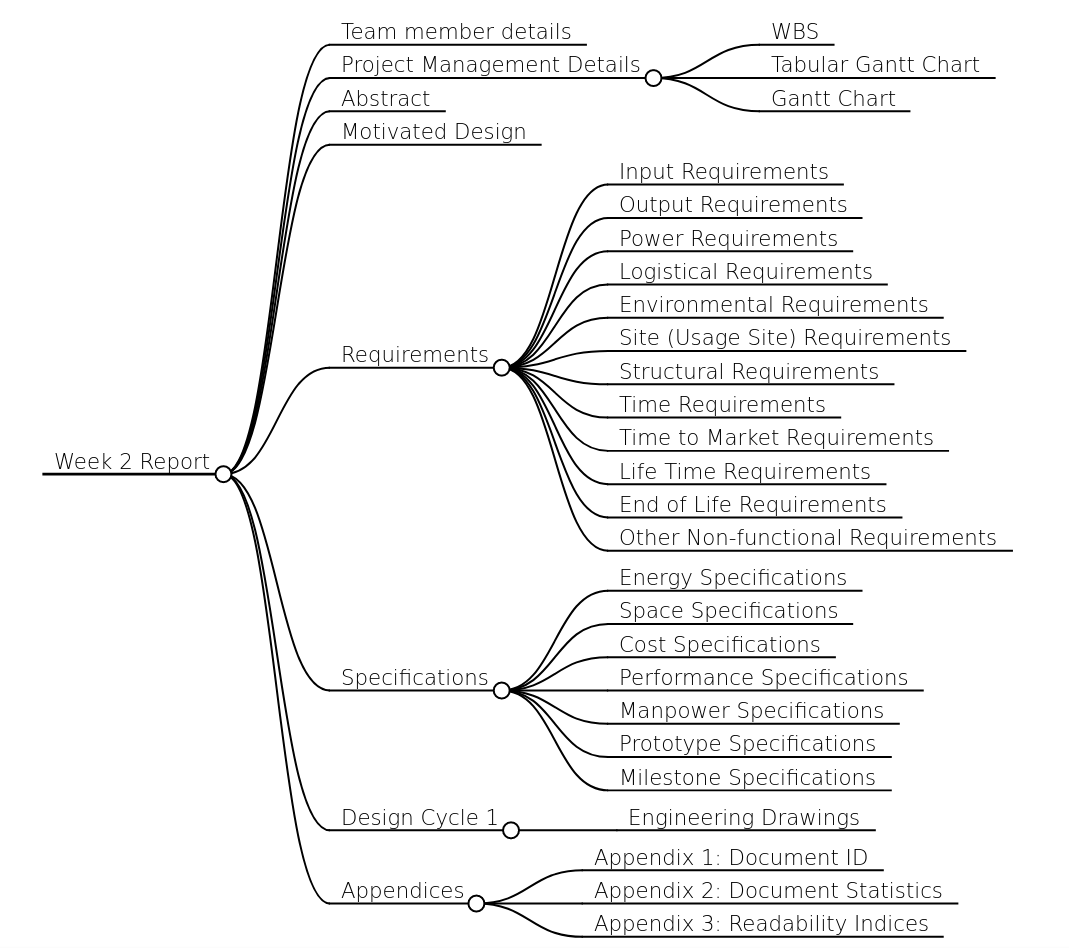
\includegraphics[scale=0.5]{mindmap}
\caption{Document Outline Mindmap}
    \label{fig:enter-label}
\end{sidewaysfigure}

\clearpage

\begin{abstract}
\addcontentsline{toc}{section}{\protect\numberline{}Abstract}
    The design document outlines a comprehensive approach to creating a cleaning machine tailored for white unbleached\index{unbleached} cotton fabric. The fabric specifications include a new, 400- \gls{thread count}, 60-\gls{Denier} cotton fabric with a dry weight of 11 kgs to be washed in a 45-minute single cleaning cycle. The machine is designed to accommodate a maximum fabric width of 2 meters, ensuring efficiency and practicality. Environmental considerations are integrated into the design, utilizing non-toxic, biodegradable\index{biodegradable} detergents for wet cleaning, aligning with sustainability standards. The machine's structural components, such as the rotating drum and water mist-steam\index{mist-steam} cleaning module, are strategically designed to optimize the \gls{Cleaning Efficacy} while preserving fabric integrity. The machine's operational features include an integrated system for introducing wet cleaning chemicals at specific stages, ensuring precise timing to maximize effectiveness while minimizing adverse effects on fabric quality. The use of a \gls{plc} and a \gls{hmi} enhances operational control and user interaction. In terms of efficiency, the \gls{tumble drying process}\cite{deans2001modelling} is highlighted, utilizing a rotating drum \cite{lim2010dynamic} with hot air circulation. The machine structure is outlined, encompassing inner and outer components, sensors, pumps, valves, and safety features. Regular cleaning and maintenance considerations are incorporated to manage lint\index{lint} buildup and ensure long-term reliability\index{reliability}. The fabric and machine specifications are meticulously addressed, considering factors such as \gls{Tear Strength}, temperature range, flammability, power load preferences, and batch size. The design emphasizes adaptability\index{adaptability} to different cleaning methods (water, dry, air) and remains cost-effective while adhering to a maximum power load of 1-phase 220V 15A or 3-phase 440V 8A.
\end{abstract}

\clearpage

\vspace{1cm}

\clearpage


\section{Project Management Details}

\begin{figure}[h!]
\centering
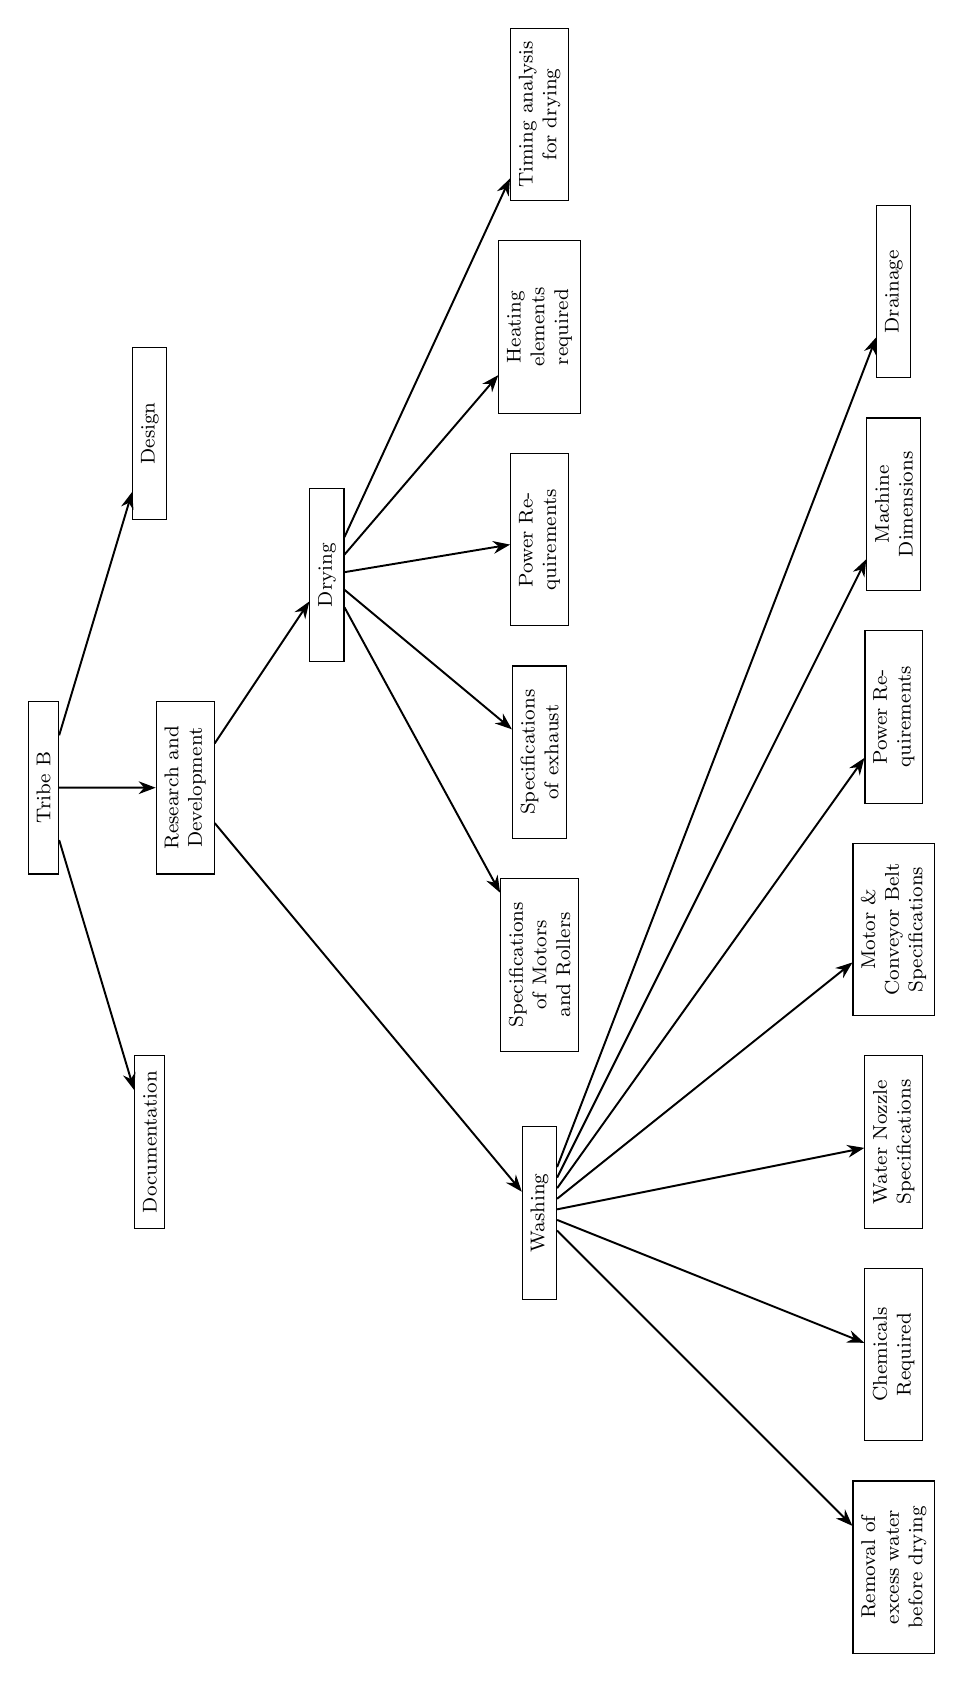
\begin{tikzpicture}[rotate=90, xscale=0.9, yscale=0.9,transform shape]

\begin{scope}[every node/.style={shape=rectangle,
    draw, align=center,
    top color=white, bottom color=white!20,font = \footnotesize,text width=22mm},
    line/.style={draw, -latex'}]
    \node (a) at (0,0) {Tribe B};
    \node (b) at (0,-2) {Research and Development};
    \node (c) at (-5,-1.5) {Documentation};
    \node (d) at (5,-1.5) {Design};
    \node (e) at (-6,-7) {Washing};
    \node (f) at (3,-4) {Drying};
\end{scope}

\begin{scope}[every node/.style={shape=rectangle,
    draw, align=center,
    top color=white, bottom color=white!20},
    line/.style={draw, -latex'},font = \footnotesize,text width=22mm]
    \node (g) at (6.5,-7) {Heating elements required};
    \node (h) at (3.5,-7) {Power Requirements};
    \node (i) at (0.5,-7) {Specifications of exhaust};
    \node (j) at (-2.5,-7) {Specifications of Motors and Rollers};
    \node (k) at (9.5,-7) {Timing analysis for drying};
    \node (l) at (-8,-12) {Chemicals  Required};
    \node (m) at (-5,-12) {Water Nozzle Specifications};
    \node (n) at (-2,-12) {Motor \& Conveyor Belt Specifications};
    \node (o) at (1,-12) {Power Requirements};
    \node (p) at (4,-12) {Machine Dimensions};
    \node (q) at (7,-12) {Drainage};
    \node (r) at (-11,-12) {Removal of excess water before drying};
\end{scope}

\begin{scope}[
              every node/.style={fill=none,circle,black},
              every edge/.style={-Stealth,draw, line width=.7pt},
			  z/.style={line width=4pt,blue!40!cyan}  
              ]
    \path [-] (a) edge node[] {} (b); 
    \path [-] (a) edge node[] {} (c); 
    \path [-] (a) edge node[] {} (d); 
    \path [-] (b) edge node[] {} (e); 
    \path [-] (b) edge node[] {} (f); 
    \path [-] (f) edge node[] {} (k); 
    \path [-] (f) edge node[] {} (j); 
    \path [-] (f) edge node[] {} (i); 
    \path [-] (f) edge node[] {} (h); 
    \path [-] (f) edge node[] {} (g); 
    \path [-] (e) edge node[] {} (l); 
    \path [-] (e) edge node[] {} (m); 
    \path [-] (e) edge node[] {} (n); 
    \path [-] (e) edge node[] {} (o); 
    \path [-] (e) edge node[] {} (p); 
    \path [-] (e) edge node[] {} (q); 
    \path [-] (e) edge node[] {} (r); 
\end{scope}
\end{tikzpicture}
\caption{\acrshort{WBS}}
\end{figure}

\clearpage

\begin{table}
\centering
\renewcommand{\arraystretch}{1.3}
\resizebox{\columnwidth}{!}{%
\begin{tabular}[scale=0.20]{|c|c|c|c|c|c|} \hline
& \textbf{Name} & \textbf{Duration} & \textbf{Start} & \textbf{Finish} & \textbf{Predecessors} \\ \hline
1 & Full Team & 10 days & 3/1/24 11:00 AM & 17/1/24 11:00 AM & None \\ \hline
2 & Team Formation \& Logistics & 1 day & 3/1/24 11:00 AM & 4/1/24 11:00 AM & None \\ \hline
3 & Requirements Question... & 2 days & 3/1/24 11:00 AM & 5/1/24 11:00 AM & None \\ \hline
4 & S1 Review & 2 days & 15/1/24 11:00 AM & 17/1/24 11:00 AM & None \\ \hline
5 & Research \& Development & 9.5 days & 5/1/24 11:00 AM & 18/1/24 4:00 PM & None \\ \hline
6 & Requirements Research & 3 days & 5/1/24 11:00 AM & 10/1/24 11:00 AM & 3 \\ \hline
7 & Specifications Research & 1.5 days & 17/1/24 11:00 AM & 18/1/24 4:00 PM & 4 \\ \hline
8 & Documentation & 7.625 days & 10/1/24 11:00 AM & 19/1/24 5:00 PM & None \\ \hline
9 & S1 Report & 1.5 days & 10/1/24 11:00 AM & 11/1/24 4:00 PM & 6 \\ \hline
10 & S1 Proofreading & 0.75 days & 11/1/24 11:00 AM & 12/1/24 9:00 AM & None \\ \hline
11 & S2 Report & 1 day & 18/1/24 4:00 PM & 19/1/24 4:00 PM & 7 \\ \hline
12 & S2 Proofreading & 0.5 days & 19/1/24 1:00 PM & 19/1/24 5:00 PM & None\\ \hline
13 & Design \& Fabrication & 0.5 days & 18/1/24 4:00 PM & 19/1/24 11:00 AM & None\\ \hline
14 & Design Finalisation \& CAD & 0.5 days & 18/1/24 4:00 PM & 19/1/24 11:00 AM & 7 \\ \hline

\end{tabular}%
}
\renewcommand{\arraystretch}{1}
\caption{Tabular Gantt Chart}
    \label{fig:enter-label}
\end{table}

\begin{figure}
\centering
\resizebox{\columnwidth}{!}{%
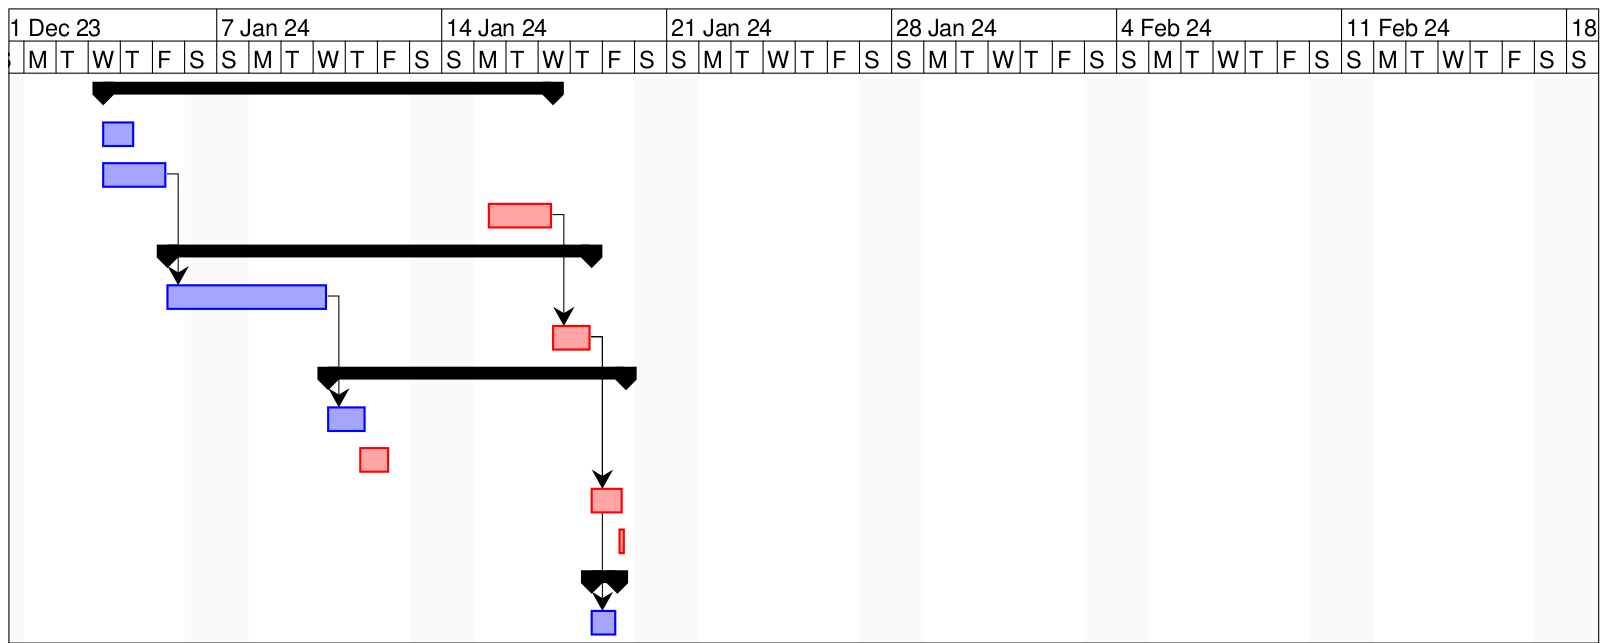
\includegraphics[trim={0 0 400 0},clip,scale=0.20]{gantt}%
}
\caption{Gantt Chart}
    \label{fig:enter-label}
\end{figure}


\clearpage

    \section{Motivated Design: Synergizing Wet Cleaning with Spray Washing}

\begin{figure*}[!b]
    \centering
    %\includegraphics{}
    

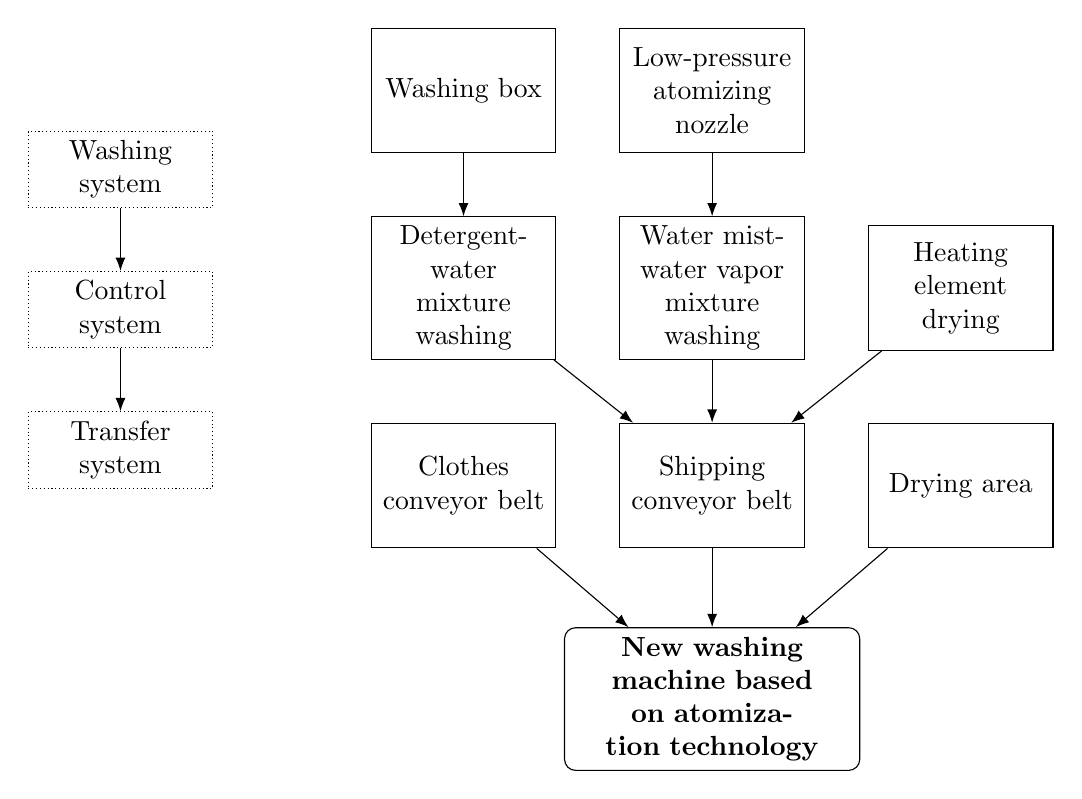
\begin{tikzpicture}[
    % Define the style for each block
    terminator/.style={rectangle, draw, text centered, rounded corners, minimum height = 5em, text width=10em},
    process/.style={rectangle, draw, text centered, minimum height = 4.5em, text width=6em},
    connector/.style={-Latex},
    smallprocess/.style={rectangle, draw, densely dotted, text centered, minimum height = 2.5em, text width=6em},
    connector/.style={-Latex},
    node distance=2cm
]

% Place nodes using explicit positioning

\node [process] (Lpan) {Low-pressure atomizing nozzle};
\node [process, left=0.8cm of Lpan] (Washingbox) {Washing box};

\node [process, below=0.8cm of Lpan] (Wmist) {Water mist-water vapor mixture washing};
\node [process, left=0.8cm of Wmist] (Detergent) {Detergent-water mixture washing};
\node [process, right=0.8cm of Wmist] (Tumbler) {Heating element drying};

\node [process, below=0.8cm of Wmist] (Ship) {Shipping conveyor belt};
\node [process, left=0.8cm of Ship] (Conv) {Clothes conveyor belt};
\node [process, right=0.8cm of Ship] (Dry) {Drying area};

\node [terminator, below=1cm of Ship] (End) {\textbf{New washing machine based on atomization technology}};

\node [smallprocess, left=2cm of Washingbox, yshift=-1cm] (Proc1) {Washing system};
\node [smallprocess, below=0.8cm of Proc1] (Proc2) {Control system};
\node [smallprocess, below=0.8cm of Proc2] (Proc3) {Transfer system};

% Draw connectors with labels
\draw [connector] (Washingbox) -- (Detergent);
\draw [connector] (Lpan) -- (Wmist);

\draw [connector] (Tumbler) -- (Ship);
\draw [connector] (Detergent) -- (Ship);
\draw [connector] (Wmist) -- (Ship);

\draw [connector] (Dry) -- (End);
\draw [connector] (Conv) -- (End);
\draw [connector] (Ship) -- (End);

\draw [connector] (Proc1) -- (Proc2);
\draw [connector] (Proc2) -- (Proc3);
\end{tikzpicture}
\caption{Machine Design Mindmap}\label{fig:enter-label}
\end{figure*}

Our inspiration for the Cotton Fabric Cleaning Machine stemmed from the client's specific need to clean new white unbleached cotton fabric, emphasizing a packaging cleaning solution for fabric manufacturers. To meet these demands effectively, our design strategically integrates the proven benefits of Wet Cleaning\index{wet cleaning} with the advanced features of Spray Washing\index{spray washing} \cite{liu2019research}.
\vspace{10pt}

Motivated by the desire to optimize stain removal, fabric preservation, and overall \gls{Cleaning Efficacy}, we seamlessly blended Wet Cleaning's non-toxic, biodegradable detergents with the precision of a Spray Washing Machine. This innovative approach not only addresses manufacturing impurities but also enhances the machine's capabilities for odor removal and environmental friendliness.
\vspace{10pt}


Understanding the importance of versatility\index{versatility}, the design accommodates various cleaning methods, including water, dry, and air, ensuring adaptability to different fabric handling needs. The motivation to adhere to power load preferences further ensures cost-effectiveness and safety in operation.
\vspace{10pt}


The user-centric design principles are rooted in the desire for efficiency and ease of operation. The 45-minute single cleaning cycle and a balanced machine size cater to the client's need for practicality and a user-friendly experience.
\vspace{10pt}


Economically driven, the design is cost-effective, aligning with budgetary constraints while adhering to environmental standards, as mandated by \acrshort{cpcb} rules. In essence, our motivation behind this integrated design is to provide a holistic fabric care solution that not only meets but exceeds client expectations through the seamless synergy of Wet Cleaning and Spray Washing technologies.




\clearpage

\section{Requirements}
\subsection{Input Requirements}

   \subsubsection{Water Requirements} To wash 11 kgs of cotton cloth, we will require around 80-90 liters of water.
   \subsubsection{Detergent Requirements} Considering an 11 kg of cotton fabric, our design recommends using 500 ml of Surf Excel Matic Front Load Liquid Detergent. With 5 liters of detergent, nearly 10-11 cotton fabrics can be efficiently washed, making it a cost-effective and resource-efficient choice.

\subsubsection{Input Requirements - Summary}
\begin{table*}[h]
\centering
\begin{tabular}{ |p{7.5cm}|p{7.5cm}| }

\hline
\textbf{Key Consideration} & \textbf{Requirement} \\
\hline
Types of stains or fabrics the machine should be optimized for & White unbleached Cotton fabric which has been just manufactured \\
\hline
The intended user of the cleaning machine & The entity who made the unbleached cotton fabric \\
\hline
Desired fiber content of the fabrics & Single ply, \gls{thread count} 400 and \gls{Denier} 60 \\
\hline
Types of yarn commonly used in the fabrics to be cleaned & Cotton yarn \\
\hline
Maximum dimensions of the fabrics that the cleaning machine should accommodate & 10 meter length x 2 meters width \\
\hline
Fabric's colorfastness\index{colorfastness} to laundering & Colours are fast, they do not run. Primarily the input is NOT coloured - white unbleached cotton cloth \\
\hline
Specific requirements for \gls{Abrasion Resistance}, especially for fabrics that may undergo frequent cleaning cycles & None. Each fabric undergoes one cleaning and is then packed \\
\hline
Minimum \gls{Tear Strength} specifications & 125 kg (\gls{Tensile Method Test}) \\
\hline
Is \gls{Seam Slippage} a critical factor, and if so, the acceptable levels for the fabrics & No, the edges of the fabric are \gls{back-folded seams} \\
\hline
Flammability\index{flammability} characteristics of the fabric & Flammable if exposed to naked flame for more than 6 seconds\\
\hline
Stains/impurity industry specifically added during the manufacturing process that need to be cleaned & No, stains are not deliberately added. Only impurities are the materials used to manufacture the cloth \\
\hline
\end{tabular}
\caption{Input Requirements}
\label{table:your_label}
\end{table*}

\subsection{Output Requirements}
  \subsubsection{Drainage System}The size of the drainage pipe is chosen based on the expected flow rate of water and chemicals during the washing process. A larger valve allows for quicker drainage, which is particularly important in a commercial setting. Size: 2-3 inches in diameter (based on flow rate calculation). Material: Stainless steel or corrosion-resistant\index{corrosion-resistant} plastic.
  \subsubsection{Ventilation} We will be using the exhaust\index{exhaust} of around 4 inches in diameter considering the \acrshort{cfm}. Approximate space that the exhaust and duct will cover is  16x16 cm.

\hspace{1cm}
\subsection{Power Requirements}
  \subsubsection{Machine Power Use} Pump for Nozzles, Motor of conveyor Belt, heating water, Control Panel(Timers, Sensors) 
Power Supply Needed - 180V - 240V
Motor for conveyor belt: 74.57 Watt
Pump for Nozzles: 1hp(745 Watt) (Approx value of power needed for pump to fulfill our need)

  
  \subsubsection{Power requirement for drying} Actual drying times and energy usage can vary based on factors such as the changing environmental factors and the moisture content of the cloth. According to our analysis of the thermodynamics of our system, the power required will be around 2000 watts.

\hspace{1cm}
\subsection{Logistical Requirements}

  \subsubsection{Adequate space for the entire machine}  The machines need sufficient space for installation and proper functioning. The assembly would require approximately an area of 3x5 meters

  \subsubsection{Water supply connection} An essential logistical requirement for the washing process, the water supply ensures the availability of the medium for \gls{wet cleaning agent}s. 80-90 Liters of water will be required for one batch

  
  \subsubsection{Ventilation for efficient drying} Proper ventilation is crucial during the drying process to facilitate the efficient removal of moisture from the fabric. 

\clearpage

\subsection{Environmental Requirements}

 \subsubsection{Good ventilation for efficient drying} Beyond its role in efficient drying, good ventilation\index{ventilation} also contributes to environmental considerations by optimizing energy efficiency during the \gls{tumble drying process}.

 
 \subsubsection{Humidity monitoring system} Machine’s efficiency depends a lot on the humidity levels so efficient humidity management through ventilation would be required

\hspace{1cm}
\subsection{Site (Usage Site) Requirements}

 \subsubsection{Well-ventilated space for drying} The drying process requires a well-ventilated space to ensure optimal conditions for moisture removal.
 
 \subsubsection{Access to water and power supply} A necessary site requirement for the washing process, ensuring a constant supply of water for the \gls{wet cleaning agent}s.
 
 \subsubsection{Proper installation of inner components in machine structures} Ensuring proper installation of inner components is vital for the overall functionality of the machines.
 
\hspace{1cm}
\subsection{Structural Requirements}

 \subsubsection{Sturdy housing\index{housing} for the spray washing machine} Sturdy housing is crucial to provide stability and durability for both machines. The rationale is to ensure the machines can withstand the mechanical movements and operational demands without compromising performance.

 
 \subsubsection{Adequate support for inner components in machine structures} Proper support for inner components is necessary to prevent malfunctions and maintain the overall integrity of the machines. The rationale is to ensure that all components are well-supported and can perform their functions optimally.

\clearpage

\subsection{Time Requirements}

 \subsubsection{Design Time Requirement} Drawing insights from prevalent industry benchmarks in designing cleaning machines for unbleached cotton fabric, our objective is to streamline the design process within a timeframe of around 4 weeks. This aims not just to meet but to surpass contemporary design efficiency, employing innovative methodologies for optimal system performance.

 
 \subsubsection{Time to Market Requirements} Comparative analysis of industry timelines underscores the variability in design-to-market durations for cleaning machines. Our commitment is to adhere to or potentially outstrip these norms, ensuring our systems reach the market promptly to address evolving demands through precision and efficient collaboration.

 
 \subsubsection{Life Time Requirements} Acknowledging the diverse operational lifespans of machines in the industry, our focal point is to gain a competitive advantage by delivering robust\index{robust} systems with prolonged operational life. Through meticulous design and stringent quality assurance, our aim is to set new industry benchmarks in system longevity\index{longevity}.
 
 \subsubsection{End of Life Requirements} In navigating the stages of disposal, recycling, and maintenance, industry practices exhibit variability\index{variability}. In our commitment to environmental responsibility, we envision surpassing standard guidelines. As the project progresses, our goal is to introduce procedures that not only meet but exceed existing industry standards, elevating the sustainability and lifecycle management of our systems.

\clearpage
\subsection{Other Non-functional Requirements}

 \subsubsection{Safety} Implementation of safety features such as emergency stop buttons and safety sensors. The rationale is to prioritize user safety\index{user safety} during the operation of the machines, minimizing the risk of accidents or malfunctions.
 
 \subsubsection{Serviceability} \gls{access panel} provided for maintenance ease. The rationale is to facilitate easy maintenance and servicing, allowing technicians or users to access internal components for repairs or cleaning without significant disruption.
 
 \subsubsection{Reliability} Consistent and reliable performance is essential for effective cleaning and drying. The rationale is to build machines that users can trust to deliver consistent results, meeting their fabric care needs reliably.
 
 \subsubsection{Efficient Water Flow Regulation} Control of water inflow and outflow for optimal usage. The rationale is to ensure that water is utilized efficiently during the washing process, contributing to resource conservation\index{conservation} and cost-effectiveness.
 
 \subsubsection{Turbidity Control} Monitoring and control of water turbidity\index{turbidity} for effective cleaning. The rationale is to maintain the clarity\index{clarity} of water during the washing process, enhancing the performance of \gls{wet cleaning agent}s and improving overall \gls{Cleaning Efficacy}.
 
 \subsubsection{Inlet and Outlet Timing} Optimal timings for water inlet and outlet during different phases of the cleaning process. The rationale is to synchronize\index{synchronize} water flow with specific stages of the cleaning cycle, optimizing the effectiveness of detergents and rinsing.
 
 \subsubsection{\acrshort{plc} for Operation Control} Use of a \acrlong{plc} for efficient operation control. The rationale is to implement advanced control systems that enhance the precision and automation of the cleaning and drying processes, ensuring consistent and controlled performance.
 
 \subsubsection{\acrshort{hmi} for User Interface and Monitoring} Incorporation of a \acrlong{hmi} for user-friendly interaction and monitoring. The rationale is to provide users with an intuitive interface to control and monitor the cleaning and drying processes, enhancing the overall user experience.
 
 \subsubsection{Environmental Considerations} The overall system design takes into account environmental impact and sustainability, incorporating elements such as biodegradable detergents, \gls{effluent treatment}, and energy-efficient processes. The rationale is to align the system with modern environmental standards and practices.
 
 \subsubsection{\Gls{effluent treatment} System} Ensures responsible management of wastewater, minimizing environmental impact. The rationale is to address environmental concerns related to wastewater disposal and contribute to sustainable and responsible fabric care practices.
 
 \subsubsection{Regular Cleaning and Maintenance Time} Design includes provisions for regular cleaning and maintenance to prevent issues such as lint buildup and ensure long-term functionality. The rationale is to promote proactive maintenance, extending the operational life of the machines and preventing potential breakdowns.


\clearpage
\subsection{Chemical Cleaning Methods Mindmap}
\vspace{0.5cm}
\begin{figure}[h]
    \centering
    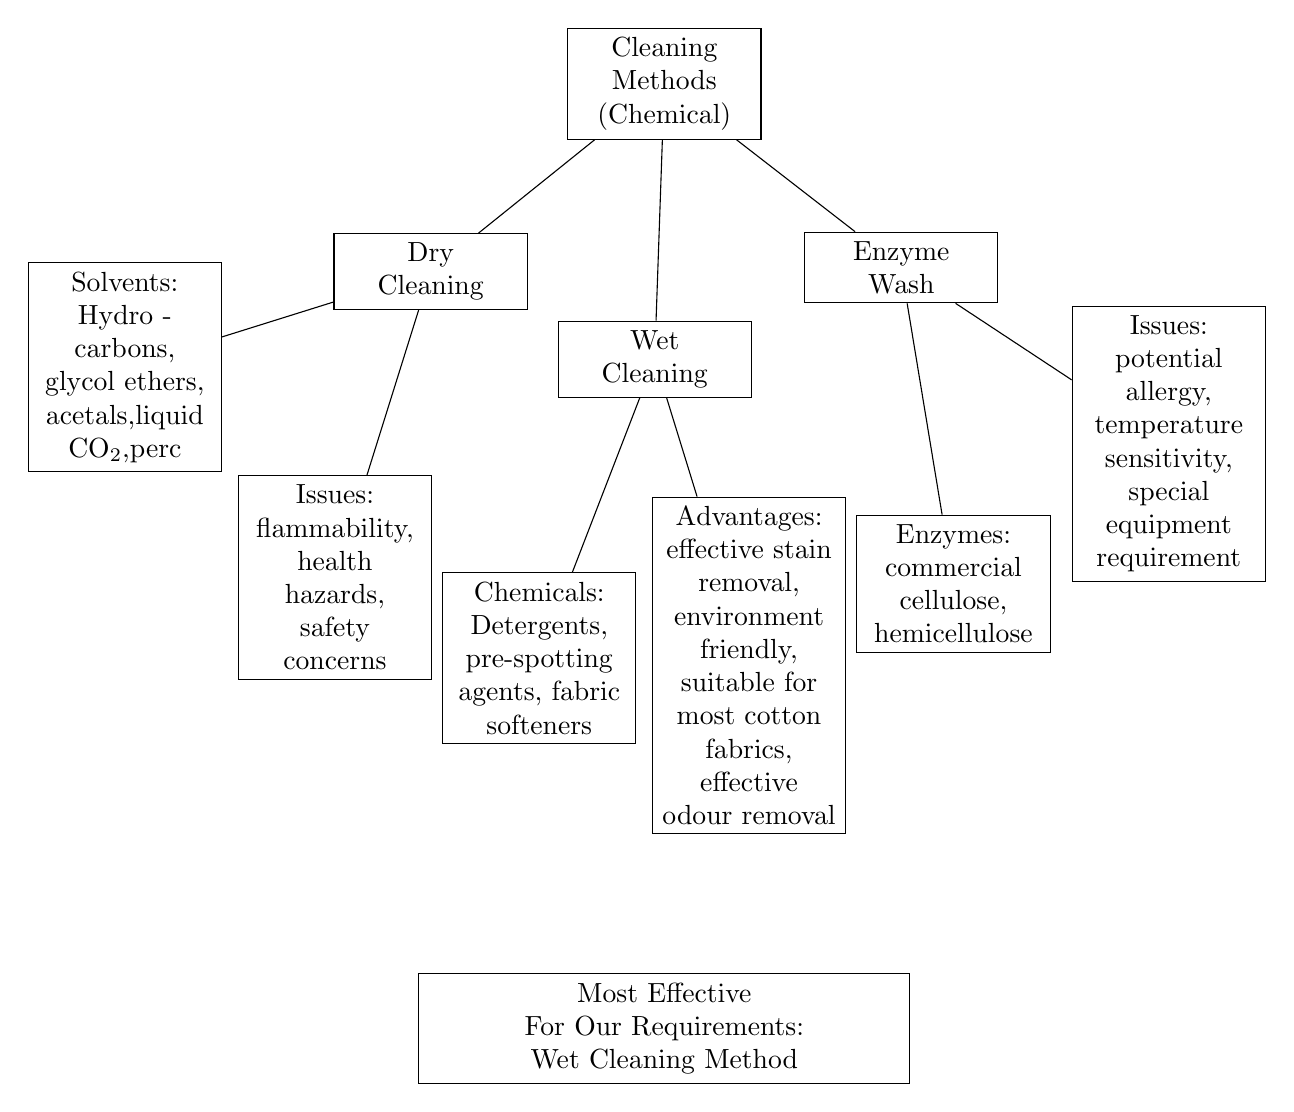
\begin{tikzpicture}[
 every node/.style = {rectangle, draw, text width=2.22cm, align = center},
 level 1/.append style = {
     level distance = 3.5cm,
     sibling angle = 120
 },
 level 2/.append style = {
     level distance =4cm,
     sibling angle = 120
 },
 level 3/.append style = {
     level distance = 4cm,
     sibling angle = 120
 }
]
 \node {Cleaning Methods \\(Chemical)}
    child [rotate=-28]{node {Dry\\Cleaning}
        child[rotate=-34] {node {Solvents: \\Hydro - carbons,\\glycol ethers,\\acetals,liquid\\CO$_2$,\acrshort{perc}}}
        child{node {Issues: \\flammability,\\health hazards, safety concerns}}
    }
    child [rotate = -2] {node {Wet\\Cleaning}
        child [rotate = -8.5] {node {Chemicals: \\Detergents,\\pre-spotting\\agents, fabric softeners}}
        child [rotate = 8.5] {node {Advantages:\\effective stain removal, environment friendly, suitable for most cotton fabrics, effective odour removal}}
    }
    child [rotate=29] {node {Enzyme\\Wash}
        child [rotate=-9] {node {Enzymes: \\commercial cellulose,\\hemicellulose}}
        child [rotate=17] {node {Issues:\\potential allergy, temperature sensitivity, special equipment requirement}}
    };
 \node at (0, -12)[text width=6cm]{Most Effective\\For Our Requirements:\\Wet Cleaning Method};
\end{tikzpicture}
    \caption{Thought process through which team narrowed down to one cleaning technique from all the possible techniques}
    \label{Chemical Cleaning Methods Mindmap}
\end{figure}



\clearpage

\section{Specifications}
\subsection{Energy Specifications}

   \subsubsection{Water Nozzles} 
   \begin{enumerate}
   \item \textbf{Pump for Nozzles:} A \SI{1}{hp} (\SI{745}{Watt}) pump is the approximate power needed to fulfill our requirements for the nozzles \cite{pearlwater_2024_kirloskar_pump}.
   \end{enumerate}

\subsubsection{Motor and Conveyor belt} 
   \begin{enumerate}
   \item The total weight to be driven by the motors is \SI{1500}{kg} and the required speed is \SI{0.25}{\m\per\min}. Assuming a coefficient of friction of 0.5, the total pull is calculated to be $1500 \times 0.25 \times 0.5 = \SI{200}{\kg\m\per\min}$ (approximately, including margin).
   \item \SI{1}{hp} is equivalent to \SI{4500}{\kg\m\per\min}.
   \item The total weight of the belt ranges from 1500-3000 kg, depending on the belt's thickness, which varies between 5 mm and 10 mm.
   \item Motor specifications range from 0.08 to 0.1 horsepower for a speed of 25 cm/min.
   \item The energy requirements are for 0.08 horsepower motors running for 45-50 minutes, resulting in an energy consumption of 0.05 kWh per motor.
   \end{enumerate}

\subsubsection{Drying} 
Actual drying times and energy usage can vary based on factors such as environmental conditions and the moisture content of the fabric. Our thermodynamic analysis suggests that the power required for drying will be around 2000 Watt \cite{ambarita_2016_clothes_drying_cabinet}.

\subsubsection{Exhaust System for Drying Chamber} 
The exhaust system requires a voltage of 240V and a power wattage of 40 Watts.

\clearpage
\subsection{Space Specifications}

   \subsubsection{Conveyor belt} 
   \begin{enumerate}
   \item The conveyor belt is made of general-purpose rubber with a density of \SI{1150}{\kg\per\cubic\m}.
   \item The length of the belt is approximately 12 meters.
   \item The width of the belt is 2.2 meters.
   \item The thickness of the belt ranges from 5 to 10 mm.
   \end{enumerate}

\subsubsection{Machine Dimensions} 
    \begin{enumerate}
        \item The machine is 2.2 meters wide.
        \item It has a height of 1 meter, with the conveyor belt approximately 0.5 meters above the ground, water nozzles and chemical sprays at a height of 0.5 meters above the conveyor belt, and the drying compartment also at 0.5 meters in height.
        \item The length of the machine is 3.5 meters, divided into a 2.5-meter conveyor belt for washing and a 1-meter long drying compartment.
    \end{enumerate}

\hspace{1cm}
\subsection{Cost Specifications}

   \subsubsection{Chemicals used for washing} 
   \begin{enumerate}
   \item For efficient and cost-effective washing, we recommend Surf Excel Matic Front Load Liquid Detergent. The estimated cost for washing one piece of clothing, including 500 ml of detergent and 300 gm of soda ash for water softening, is Rs 142 \cite{leverette_2023_detergent}.
   \item With 5 L of detergent, approximately 10-11 cotton fabrics can be washed. The cost of 500 ml Surf Excel Matic detergent is Rs 130. Therefore, the cost requirement for 10 such clothes would be Rs 1300.
   \item For 1 piece of clothing: 500 ml of liquid detergent + 300 gm of soda ash, the total cost is Rs 130 + Rs 12 = Rs 142.
   \end{enumerate}

\subsubsection{Water Nozzles} 
The cost of water nozzles ranges from Rs 300-500 per nozzle \cite{lechler_2024_nozzles_washing}.

\subsubsection{Motor and Conveyor Belt} 
   \begin{enumerate}
   \item The cost of the belt is Rs 4500 per meter (2 meters wide), totaling Rs 50,000 for 10-11 meters.
   \item The cost of a motor is Rs 5000 \cite{exportersindia_2024_induction_motor}.
   \end{enumerate}

\subsubsection{Heating Element Cost} 
Nichrome is a cost-effective heating element, offering a balance between efficiency and affordability, with an estimated cost of Rs 1800 per kg \cite{wise_answer_2024, indiamart_2024_nichrome}.

\subsubsection{Rollers Cost} 
The cost for rollers is Rs 15,000 per piece, with the price varying depending on the diameter. We require stainless steel rollers due to their corrosion resistance and good mechanical properties over a wide range of temperatures \cite{indiamart_2024_stainless_steel_rolls}.

\subsubsection{Exhaust Cost} 
The exhaust costs around Rs 1800, and the duct made of aluminum will cost Rs 720.

\subsubsection{Assembly Cost} 
The aluminium body around Rs 6000, and the cost of fittings and other components will be around Rs 2500.

\subsubsection{Software Cost} 
Our team uses FreeCAD for both CAD drawings and simulations, resulting in zero software costs.

\subsubsection{Total estimated cost for machines}
\begin{enumerate}
    \item  7-8 nozzles for washing and 7-8 nozzles for rinsing along with 5 sprinklers for chemical action cost 20*500 = 10000 Rs
    \item 2 Rollers of diameter 21 cm (For conveyor belt for washing) and 5 rollers of diameter 9 cm (For conveyor belt for drying) together cost 15*2 + 3*5 = 45000 Rs
    \item The conveyor belt for washing (5m) along with the conveyor belt for drying (square root(5) + 1 m = Approximately 3.25m) cost around 38000 Rs
    \item Exhaust, heating elements and duct Cost approximately 6000 Rs
    \item 2 Motors for the two conveyor belts together cost 2*5000 = 10000 Rs
    \item Final assembly cost 6000+2500 = 8500 Rs
\end{enumerate}


\clearpage
\subsection{Performance Specifications}
   \subsubsection{Chemicals used for washing}
   \begin{enumerate}
   \item \textbf{Soft or Hard Water Considerations:} To address water hardness, our design incorporates soda ash for effective water softening. Estimations for soda ash usage are tailored to the water hardness levels to ensure optimal washing performance \cite{cleanwaterstore_2024_hardness}.
   \item \textbf{Estimation for soda ash usage:} Depending on the water hardness, ranging from light to hard, we adjust soda ash usage accordingly, with a price of Rs 40 per kg.
   \item \textbf{Safety Standards and Environment Guidelines:} Our washing machine design adheres to safety and environmental sustainability standards, ensuring compatibility with Surf Excel detergent \cite{unilever_2024_safety_environment}.
   \end{enumerate}

\subsubsection{Water Nozzles} 
\begin{enumerate}
\item \textbf{Nozzles for the main wash:} High-impact flat fan nozzles or tongue-type nozzles are recommended for the main wash. The spray angle should be 30 to 45 degrees, ensuring a sharp jet suitable for low pressure. These nozzles have a longer service life due to their hardened nozzle mouthpiece \cite{lechler_2024_nozzles_washing}.
\item \textbf{Nozzles for rinsing:} Rinsing requires nozzles that produce small droplets for quick runoff. Flat fan nozzles with a very low flow rate are suitable for this stage.
\end{enumerate}

\subsubsection{Drying}
The total heat required to turn m mass of water (in Kg) into water at 100 degrees is ms(100-20) (Where s is the specific heat capacity of water, assuming that after washing, the water temperature is 20 degrees Celsius.) To turn it into steam, we need an extra mL Joules of Energy, where L is the latent heat of vaporization. As we use sponge rollers before they enter the drying chamber, which squeezes out most of the water, let's assume the worst case, where 5 kg of water is left back on an 11 Kg dry cloth. The total energy required is: 5000*4.186*80+5*2.25*10\^6 = 12924400 J or 12,924.4 kJ. For time, divide this by the power the heating element provides, which is 5 Kilo Watts. So, the total time required is 12,924.4/5 sec., i.e. Approx 43 Mins.

\subsubsection{Drainage System}
   \begin{enumerate}
   \item \textbf{Valve Size:} The valve diameter should be 2-3 inches, made of stainless steel or corrosion-resistant plastic, and located at the lowest point downstream of the wash chamber.
   \item \textbf{Material and Durability:} The drainage system should use \acrshort{hdpe} or \acrshort{pvc} materials with a diameter matching the valve size, sloped towards the valve for efficient drainage.
   \item \textbf{Parameters for Drainage System Design:} The design should account for residential and commercial flow rates, with a focus on peak flow handling and accessibility for maintenance.
   \end{enumerate}


\clearpage

\subsection{Manpower Specifications}
The tribe coordinators spent around 18 hours each in this week's submission coordinating with the different teams and reviewing their work.
\begin{table}[h]
\centering
\begin{tabular}{|c|c|c|}
\hline
Name & Entry No. & Working Hours \\
\hline
Bhumi Gadhavi & 2021MT60950 & 8 \\
Tanmay Jhalani & 2021EE30389 & 1 \\
Shantanu Pandit & 2021MT10252 & 1 \\
Pramsu Shrivastava & 2021EE10140 & 5 \\
Parth Naikwad & 2021EE10672 & 5 \\
Yash Bafna & 2021EE10660 & 1 \\
Abhay Yadav & 2021EE10151 & 5 \\
Ram Gopal Chaudhari & 2021EE10671 & 1 \\
Vivek Pratap Singh & 2021EE10687 & 5 \\
Shreya Gupta & 2021MT10906 & 3 \\
Vaibhav & 2021EE10641 & 5 \\
Devanshu Ataria & 2021EE10162 & 5 \\
Anmol Bansal & 2021EE10643 & 5 \\
Vedant Patel & 2020EE10520 & 1 \\
Aditi Srivastava & 2021MT10228 & 1 \\
Anusha Kedawat & 2021EE30718 & 1 \\
Manan Singal & 2021EE10138 & 1 \\
Tanisha Chouhan & 2021EE10693 & 1 \\
Vedant Kokate & 2021EE10631 & 5 \\
Subham & 2022MT11823 & 5 \\
Himanshu Ghusinga & 2021MT10936 & 1 \\
Ranjeet Mishra & 2021EE10656 & 1 \\
Siddharth & 2022MT62028 & 3 \\
\hline
\end{tabular}
\caption{Design Team work-hour estimation}
\label{tab:teamDetails}
\end{table}

\begin{table}[h]
\centering
\begin{tabular}{|c|c|c|}
\hline
Name & Entry No. & Working Hours \\
\hline
Keshav Singhal & 2021EE10788 & 15 \\
Advait Prashant Rege & 2021MT60946 & 15 \\
Rishika Goel & 2021EE30725 & 6 \\
Ridhima Gupta & 2021EE30719 & 8 \\
Diksha & 2021EE30717 & 8 \\
Tushar Daima & 2021EE10688 & 8 \\
Ridam Kumari & 2021EE10158 & 8 \\
Harsh Bagde & 2021EE10690 & 8 \\
Nidhish & 2021EE30176 & 4 \\
Priyal Jain & 2021MT60949 & 7 \\
Aditya Thomas & 2021MT60944 & 7 \\
Pratibha Patel & 2021EE10681 & 8 \\
Divyansh Bhatnagar & 2021EE30721 & 8 \\
Siddhika Tailor & 2021EE10683 & 8 \\
Narendra Nath Sharma & 2021EE10695 & 4 \\
Stuti Anand & 2021EE30748 & 6 \\
Anish Gupta & 2021EE10663 & 7 \\
Dhruv Mittal & 2021EE10626 & 8 \\
Mridul Jagrat & 2021EE30182 & 7 \\
Abhishek Meena & 2021EE10172 & 4.5 \\
Kinshuk Bansal & 2021EE30701 & 2 \\
\hline
\end{tabular}
\caption{Research Team work-hour estimation}
\label{tab:teamDetails}
\end{table}

The research team members gave an average of 8 hours for this week's submission. The work included researching on the assigned topics by the activity coordinator and then presenting and refining their work to finalise the machine specifications. These 8 hours also include the time spent in meetings and generating Zotero files for the final submission. The activity coordinators spent around 15 hours on the submission. We have 19 members and 2 activity coordinators in the research team, so the man hours is nearly 182 for the research team.
\\Competency/ skillset required- The research team members required excellent comprehension skills to be able to enhance the reading capabilities of the tribe. They were also required to learn to generate their references using Zotero. The design team was divided into subteams, electrical and mechanical. The electrical subteam was trained for Arduino programming, PCB designing and soldering. The mechanical team was trained for CAD designing in FreeCAD and laser cutting.
\\Surplus manpower-During the initial days only some of the members of design team were collaborating with the research team to come up with the final design for the cleaning machine while the others were underutilised. However towards the end they were fully involved with the freeCAD designing of the final assembly.

\begin{table}[h]
\centering
\begin{tabular}{|c|c|c|}
\hline
Name & Entry No. & Working Hours \\
\hline
Shourya Vir Jain & 2022EE31798 & 3 \\
S Anuj Karthik & 2021EE10667 & 2.5 \\
Shreya Singla & 2020EE10671 & 3 \\
Gourab Raj Sabat & 2022EE11675 & 3 \\
Ashi Veerman & 2021MT10241 & 3 \\
Bhargab Sonowal & 2021MT10937 & 3 \\
Rakshitha & 2021MT10904 & 2.5 \\
Sanju N S & 2021EE30732 & 2.5 \\    
Dhruv Joshi & 2022EE32079 & 3 \\
Drishti Gupta & 2021EE10649 & 3 \\
Praveen Kumar Srivastava & 2021EE10133 & 0 \\
Deepak Kumar & 2021EE10152 & 0 \\
Varshith Reddy Ryala & 2021EE10142 & 2.5 \\
Raswanth J & 2021EE30179 & 3 \\
Prisha Jain & 2021EE30330 & 2.5 \\
Garv Gupta & 2021MT60953 & 2.5 \\
Sanjay Karela & 2012MT50616 & 0 \\
Dhruv Nagpal & 2020EE11013 & 3 \\
\hline
\end{tabular}
\caption{Documentation Team work-hour estimation}
\label{tab:teamDetails}
\end{table}





\clearpage

\subsection{Prototype Specifications}
Because of the limitations of available smaller standard parts, a lot of the dimensions could not directly be scaled down by a factor of 10.
    
    \subsubsection{Motor}
    We are assuming (1/100) volume and weight of our machine, as per our dimensionality calculations. 
    \begin{enumerate}
    \item The total weight being driven is \SI{2}{\kg\m\per\min}
   \item The total weight of the belt ranges from 15-30 kg.
   \item The motor will run at 0.001 horsepower.
   \item The energy requirements are for 0.0005 kWh per motor.
   \end{enumerate}

   \subsubsection{Drying}
    The power required for drying will be around 500 - 800 watts.
    \subsubsection{Exhaust}
    The exhaust system requires a voltage of 240V and a power wattage of 10 - 16 Watts.

    \subsubsection{Conveyor belt} 
   \begin{enumerate}
   \item The conveyor belt is made of general-purpose rubber with a density of \SI{1150}{\kg\per\cubic\m}.
   \item The length of the belt is 2 meters due to a larger estimation of washing and drying size.
   \item The width of the belt is 26 centimetres to leave slack for cloth.
   \item The thickness of the belt ranges from 3 to 5 mm.
   \end{enumerate}

\subsubsection{Machine Dimensions} 
    \begin{enumerate}
        \item The machine is 26 centimetres wide.
        \item The height of the conveyor belt is 30 centimetres.
        \item The length of the machine is 70 centimetres, divided into a 50-centimeter conveyor belt for washing and a 20-centimeter-long drying compartment.
    \end{enumerate}

    \subsubsection{Chemicals cost}
   We will use 50 millilitres of detergent and 30 grams of soda leading to a cost of 14.2 rupees.
   \subsubsection{Heating elements cost}
   The cost of heating elements will be 1800 rupees per kilogram.
   \subsubsection{Drainage System Performance}
    \begin{enumerate}
   \item The valve diameter should be 2-3 centimetres.
   \item There will be a  use of 2 - 4 centimetres of material with the same diameter as the valve.
   \item The chosen flow rate is 50 litres per minute.
   \end{enumerate}

\clearpage

\begin{table}[t]
\centering

\begin{tabularx}{\textwidth}{|c|X|c|} \hline
\textbf{Milestone} & \textbf{Description} & \textbf{\acrshort{TRL}} \\ \hline
1 & Practical applications can be invented once basic principles are observed. & \acrshort{TRL}-2 \\ \hline
2 & Active research and development is initiated, including analytical studies and laboratory studies. & \acrshort{TRL}-3 \\ \hline
3 & The basic components of the technology are integrated to establish that the pieces will work together. & \acrshort{TRL}-4 \\ \hline
4 & Representative model or prototype system is tested in a relevant environment. & \acrshort{TRL}-6 \\ \hline
\end{tabularx}

\caption{Milestone \acrshort{TRL} Levels}
\end{table}

\subsection{Milestone Specifications} 
    \subsubsection{Milestone 1} Develop a comprehensive \gls{cad} model that precisely outlines the trajectory\index{trajectory} of the cloth within the cleaning machine. \\ 
    \textbf{\acrshort{TRL}-2:} Practical applications can be invented once basic principles are observed.
    \subsubsection{Milestone 2}⁠ Refine the \acrshort{cad} design to incorporate well-defined structures for seamless integration of auxiliary\index{auxiliary} components, such as water and chemical inputs, and an efficient drainage system. \\ 
    \textbf{\acrshort{TRL}-3:} Active research and development is initiated, including analytical studies and laboratory studies.
    \subsubsection{Milestone 3} Synthesize the comprehensive \acrshort{cad} model with the intricate electrical system and circuitry required for the cleaning machine. Electrical assembly and designing of \acrshort{hmi}. \\ 
    \textbf{\acrshort{TRL}-4:} The basic components of the technology are integrated to establish that the pieces will work together.
    \subsubsection{Milestone 4} Fabricate the final prototype\index{prototype} of the cleaning machine, incorporating all finalized \acrshort{cad} designs and electrical components.\\ 
    \textbf{\acrshort{TRL}-6:} Representative model or prototype system is tested in a relevant environment.

\clearpage
\section{Design Cycle 1 - Engineering Drawings}

The main components of our machine include the following:
\begin{enumerate}
    \item \textbf{Nozzle} - The component that directs the flow of water.
    \item \textbf{Washing Conveyor} - This moves the laundry through the wash cycle.
    \item \textbf{Drying Conveyor} - Responsible for the removal of moisture post-wash.
    \item \textbf{Final Assembly} - Where all parts are assembled into the final product.
\end{enumerate}
Detailed drawings of these components are presented from the next page.

\begin{sidewaysfigure}[h!]
    \centering
\includesvg[width=\columnwidth]{Nozzle}
\caption{Engineering Drawing for Nozzle}
\end{sidewaysfigure}

\clearpage

\begin{sidewaysfigure}[h!]
    \centering
\includesvg[width=\columnwidth]{Washing Conveyor}
\caption{Engineering Drawing for Washing Conveyor}
\end{sidewaysfigure}

\clearpage

\begin{sidewaysfigure}[h!]
    \centering
\includesvg[width=\columnwidth]{Drying Conveyor}
\caption{Engineering Drawing for Drying Conveyor}
\end{sidewaysfigure}

\clearpage

\begin{sidewaysfigure}[h!]
    \centering
\includesvg[width=\columnwidth]{Assembly}
\caption{Engineering Drawing for Assembly}
\end{sidewaysfigure}

\clearpage

\begingroup
\let\oldthesection\thesection
\addtocounter{section}{+1}
\addcontentsline{toc}{section}{\protect\numberline{\thesection}References}
\let\thesection\oldthesection 
\endgroup


\bibliography{ref}

\clearpage
\section*{}
\addcontentsline{toc}{section}{\protect\numberline{}Abbreviations}
\printglossary[type=\acronymtype]

\clearpage
%Glossary should be at the end of document according to the format that sir sent

\section*{}
\addcontentsline{toc}{section}{\protect\numberline{}Glossary}
\printglossary

\clearpage

\printindex
\clearpage

\begin{appendices}
\section{Appendix 1: Document ID}
   \begin{enumerate}
       \item Document Type: Private Release 
       \item Document Authorised by: Subrat Kar, Instructor (\href{mailto:subrat@ee.iitd.ac.in}{subrat@ee.iitd.ac.in})
       \item Publication Date: 13 Jan 2023
       \item Version Number: 1.4
       \item Github Repository Details: \href{https://github.com/jdhruv1503/elp305-tribe-b-submission-2-page}{jdhruv1503/elp305-tribe-b-submission-2-page}
   \end{enumerate}

\section{Appendix 2: Document Statistics}
    \begin{itemize}
       \item Word Count: 7993
       \item Number of Sentences: 1139
       \item Number of Characters: 41089
    \end{itemize}
    
\section{Appendix 3: Readability Indices}
    \begin{itemize}
        \item \textbf{Readability Index\footnote{The readability index indicates the approximate reading grade level of a text based on the US education system. The formula takes into account characters in a given word and the words in a given sentence. It varies from 0 - 16+.}:} 3.3 
        \\This means that this text can be understood by children who can read books with chapters. 
        \item \textbf{Gunning-Fog Index\footnote{On a scale from 0 -20, the Gunning-Fog Index is a weighted average of the number of words per sentence and the number of long words per word. This can be understood as the text can be understood by someone who left full-time education at a later age than the index. Hence a lower Gunning-Fog index is easier to read.}:} 8.1 
        \\This means that the text can be easily understood by someone who has passed grade 8, US education standards.
        \item \textbf{Flesch Reading Ease\footnote{The Flesch Reading Ease indicates the approximate reading grade level of a text. The formula takes into account sentence length and word length. It is based on a 0-100 scale. A high score means that the text is easier to read.}:} 57.1 \\This means that this text can be understood by 12-13 year olds.
        \item \textbf{Coleman Liau Index\footnote{On a scale of 0 - 17+, the Coleman Liau Index relies on characters and calculates the index based on the number of characters in a word and the number of words in a sentence. The score of the text indicates the US school level a person needs to understand the text.}:} 10.1 
        \\This means that the text can be easily understood by someone who has passed grade 10, US education standards.

    \end{itemize}
\end{appendices}
\clearpage

\end{document}
